\chapter{Einführung}
\section{Aufgabenstellung}
Ziel dieses Praktikums war es eine Software zu konstruieren um \QRCodes in Bildern zu lokalisieren und danach als Binärbild zu extrahieren.
Dabei sollten sich die Teams auf \QRCodes, die dem ISO/IEC Standard 18004 entsprechen, beschränken.
Unter der Annahme, dass sämtliche \QRCodes auf den Eingabebildern planar sind, sollten perspektivische Transformationen oder ähnliche Verzerrungen entfernt werden.
Zusätzlich sollte sich jedes Team darum kümmern ein \emph{Dataset} zur Analyse und späteren Evaluation zu erschaffen.
 
\section{Aufbau des \QRCodes}
Um das spätere Vorgehen der Lokalisierung des \QRCodes nachvollziehen zu können, wollen wir kurz auf einen Teil des Aufbau des \QRCodes eingehen, der für die folgende Arbeit von Bedeutung ist.
Jeder \QRCode besteht aus drei \emph{\fps} (siehe Abbildung \ref{fig:strukturqrcode} Muster 4.1) welche in der oberen linken, oberen rechten und unteren linken Ecke angeordnet sind und sowohl zur Lokalisierung und Rotation verwendet werden. Zwischen den \fps befinden sich die \emph{Timing Patterns} (siehe Muster 4.3), welche aus abwechselnd \glqq schwarz - weißen\grqq\ Punkten (\emph{Module}) bestehen.

\begin{figure}[h]
\centering
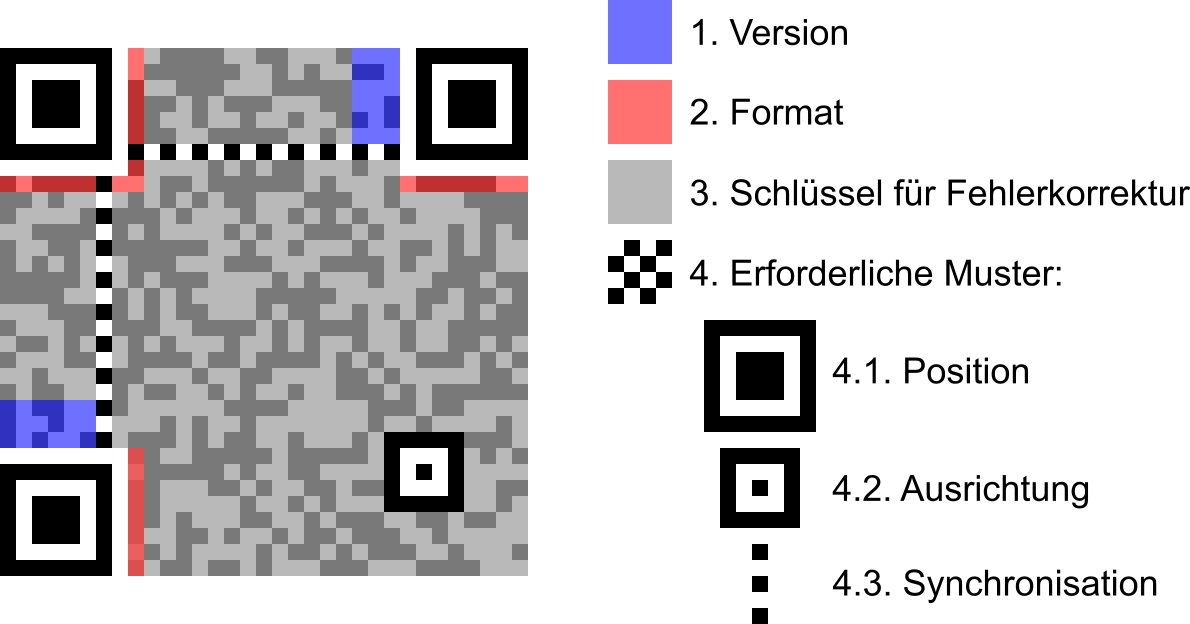
\includegraphics[scale=0.27]{images/QR_Code_Struktur_Beispiel.png}
\caption{\QRCode Strukturbeispiel (siehe Quelle \cite{qrcoderef})}
\label{fig:strukturqrcode}
\end{figure}

Zusätzlich gibt es noch \emph{Alignment Patterns} (Muster 4.2), Versions- und Formatinformationen, welche hier in Rot und Blau gekennzeichnet sind. Diese werden im Verlauf dieser Arbeit aber nicht verwendet. Die eigentliche kodierte Nachricht ist in Grau dargestellt.

Die Größe der \QRCodes ist beschränkt durch die Anzahl der \emph{Module}. Die Anzahl der \emph{Module} liegt zwischen $21 \times 21$ und $177 \times 177$. Beispielsweise sei der Code in Abbildung \ref{fig:strukturqrcode} einer der Größe $21 \times 21$. Dann hätte ein \emph{\fp} die Länge von $7$ \emph{Modulen}. Die Anzahl ergibt sich aus der einzigartigen $1:1:3:1:1$ Struktur eines \emph{\fps}. Dieser Aufbau wird später für die Rasterisierung des \QRCodes verwendet.

\section{Die verwendete Bibliothek OpenCV}
\OpenCV\cite{opencv} ist eine Bibliothek mit Algorithmen spezialisiert auf \glqq Computer Vision\grqq . Sie wurde für die Programmiersprachen C/C++ geschrieben und steht unter BSD Lizenz. Es gibt mehrere Versionen der Bibliothek, die aktuellste ist die Version 3.2. Das implementierte Programm setzt die Mindestanforderung auf Version 2.4. Außer \OpenCV wird keine weitere Bibliothek verwendet.